Several approaches can be used for classifying time series data. Unsupervised learning methods such as k-means clustering are commonly used when the structure of the data is unknown. These methods can capture complex patterns but are often less interpretable. Alternatively, statistical approaches based on hypothesis testing provide more transparent decision rules but may rely on stronger assumptions about the data. \\

In this study, the objective is to separate cells into two classes, seasonal and non-seasonal. Given the binary nature of the problem and the need for interpretability, a simple and explainable approach is preferred over more complex clustering methods. \\

To identify a simple and interpretable seasonal indicator, a binary feature based on public school holiday schedules in Copenhagen [reference] was constructed. Each time series was labeled as either occurring during a holiday period or a non-holiday period. \\

For each cell, the traffic data was divided into two groups corresponding to holiday and non-holiday periods. The average traffic volume was then computed for both groups. To obtain an overall overview at the site level, the average values across all cells within each site were visualized using boxplots, as shown in Figure \ref{fig:box_plot_holiday_avg_site}. \\


\begin{figure}[h]
    \centering
    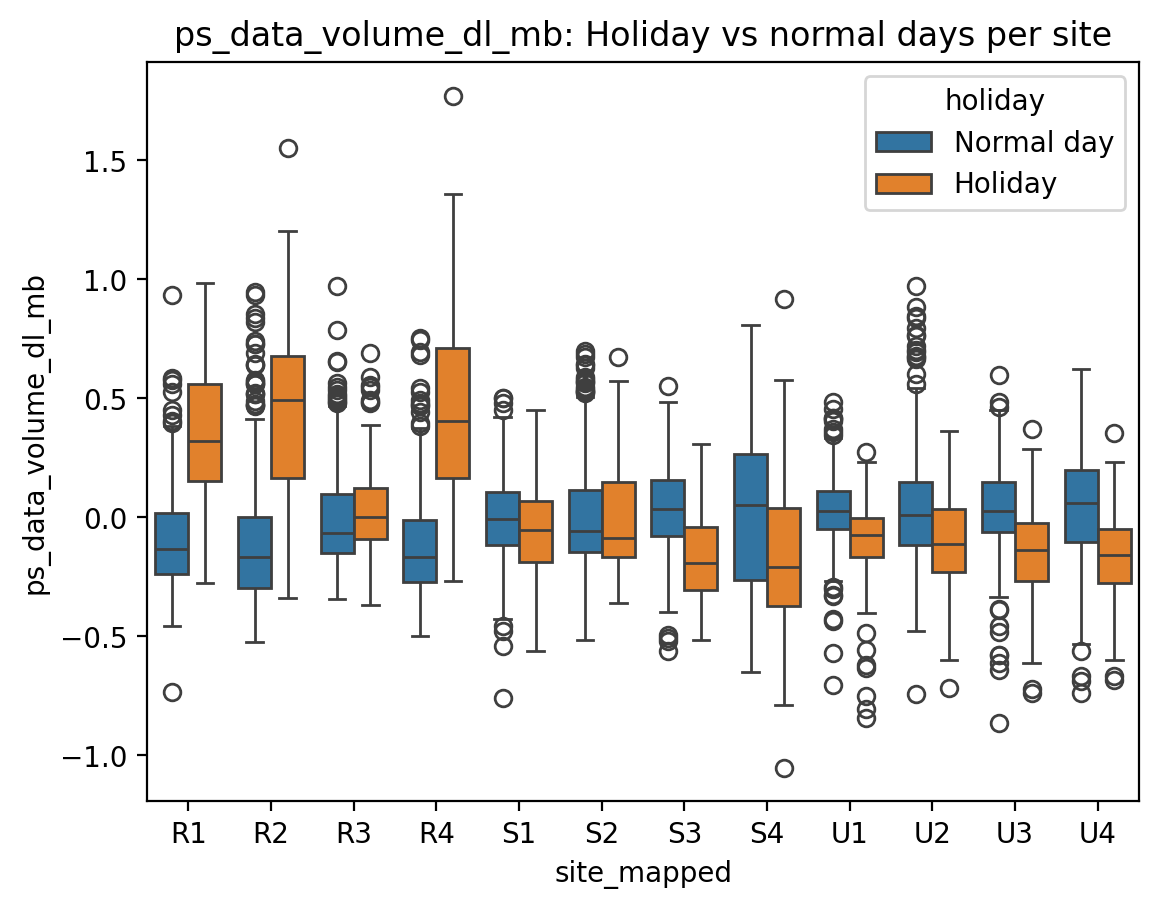
\includegraphics[width=\linewidth]{figures/box_plot_holiday_avg_site.png}
    \caption{T-test holiday volume vs non-holiday volume for all individual cells}
    \label{fig:box_plot_holiday_avg_site}
\end{figure}

Figure \ref{fig:box_plot_holiday_avg_site} shows differences in standardized traffic levels between holiday and non-holiday periods across site categories.

Recreational sites (R1--R4) show a consistent positive shift in standardized traffic during holiday periods. The mean difference between holiday and non-holiday periods ranges from $0.04$ to $0.58$ standard deviations. The strongest effects are observed at R4 ($\Delta = 0.582$) and R2 ($\Delta = 0.547$), followed by R1 ($\Delta = 0.442$). R3 shows only a weak shift ($\Delta = 0.051$), indicating a much smaller seasonal response compared to the other recreational sites. \\

Urban sites (U1--U4) show a consistent negative shift during holiday periods. Mean differences range from $-0.13$ to $-0.20$ standard deviations, with the strongest decreases observed at U4 ($\Delta = -0.202$) and U2 ($\Delta = -0.192$). This indicates lower standardized traffic levels during holidays compared to normal days across all urban locations. \\

Suburban sites (S1--S4) show mixed and weaker effects. S1 ($\Delta = -0.039$) and S2 ($\Delta = -0.020$) show near-zero changes, indicating little difference between holiday and non-holiday periods. S3 ($\Delta = -0.213$) and S4 ($\Delta = -0.141$) show larger negative shifts, more similar to urban patterns. Overall, the suburban group shows higher diversity, with no consistent directional response across all sites. \\

Median differences follow a similar pattern, with recreational sites showing positive shifts and urban sites showing negative shifts, confirming that the observed effects are not driven solely by extreme values.
\subsection{T-test Validation}
The boxplot analysis demonstrates that holiday periods produce different traffic volumes depending on site category, suggesting that the holiday indicator can serve as a basis for statistical classification at the cell level. To formalize this, an independent two-sample t-test is applied to each cell individually, testing whether the mean traffic volume during holiday periods differs significantly from that during non-holiday periods. \\

The t-statistic is defined as:

\begin{equation}
    t = \frac{\bar{x}_1 - \bar{x}_2}{\sqrt{\dfrac{s_1^2}{n_1} + \dfrac{s_2^2}{n_2}}}
    \label{eq:ttest}
\end{equation}

where $\bar{x}_1$ and $\bar{x}_2$ are the sample means, $s_1^2$ and $s_2^2$ are the sample variances, and $n_1$ and $n_2$ are the number of observations in the holiday and non-holiday groups. \\

The t-test is well suited to this problem for several reasons. First, the two groups, holiday and non-holiday periods, are naturally defined and non-overlapping. Second, the test provides a statistical measure of whether the difference in mean traffic between the two groups is likely to occur by chance. Based on this, a simple decision rule is introduced, cells with statistically significant differences in mean traffic ($p < 0.05$) are labeled as seasonal, while the remaining cells are labeled as non-seasonal. This produces an interpretable and reproducible classification criterion without requiring manual threshold tuning. \\

\begin{figure}[h]
    \centering
    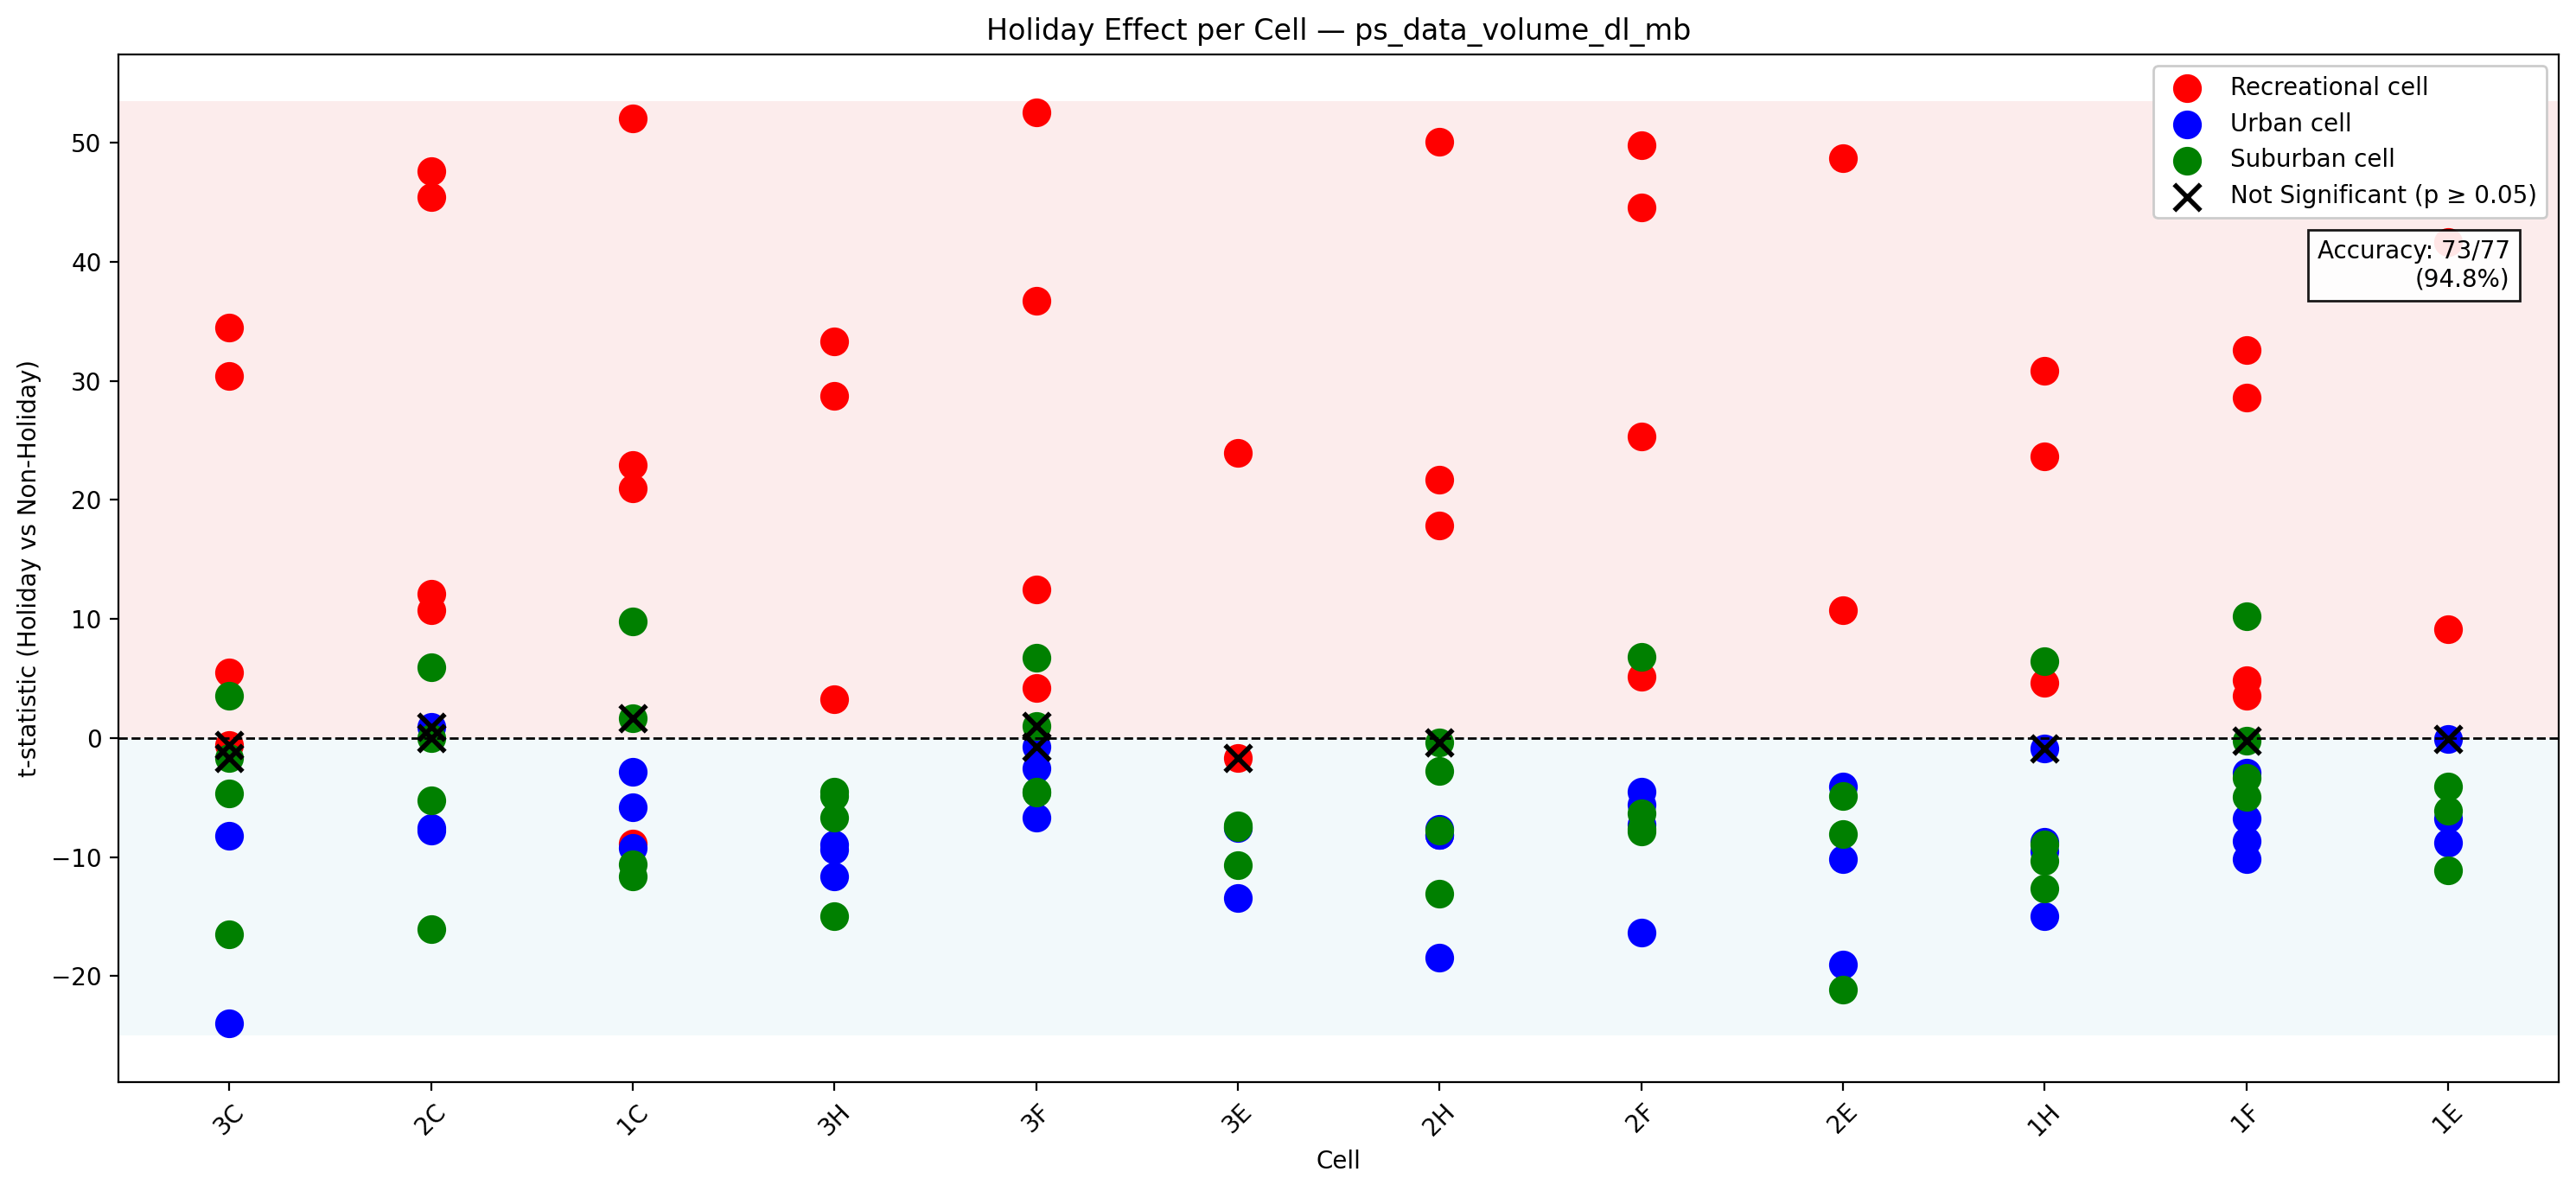
\includegraphics[width=\linewidth]{figures/t_test_all_cells.png}
    \caption{T-test holiday volume vs non-holiday volume for all individual cells}
    \label{fig:t_test_all_cells}
\end{figure}

Figure \ref{fig:t_test_all_cells} shows the t-test results across all individual cells. A clear separation is observed, with the majority of cells belonging to recreational sites identified as seasonal, while urban cells are predominantly identified as non-seasonal. This alignment with the geographic site categories suggests that the method captures meaningful differences in traffic behavior without using geographic location as an input. \\

The suburban sites present a more mixed case, as their traffic behavior does not conform as clearly to either category. Cells from suburban sites are distributed across both classes, reflecting the mixed nature of these environments. Because the method produces consistent results for both recreational and urban sites, it provides a useful basis for analysing suburban cells, where no clear ground truth classification exists. This highlights the value of a data driven approach over simple geographic labeling, as it can distinguish cases where location alone is not enough to determine traffic behavior. \\